\documentclass{beamer}
\usetheme{Singapore}

\title{Deep Deterministic Policy Gradient (DDPG) for Atari Galaga}
\subtitle{CS4100 Project Proposal}
\author{Thomas Wilson}
\institute{Khoury College of Computer Sciences}
\date{\today}

\begin{document}
\begin{frame}
	\titlepage
\end{frame}

\begin{frame}
	\frametitle{Policy Gradient Methods}
	\center 
	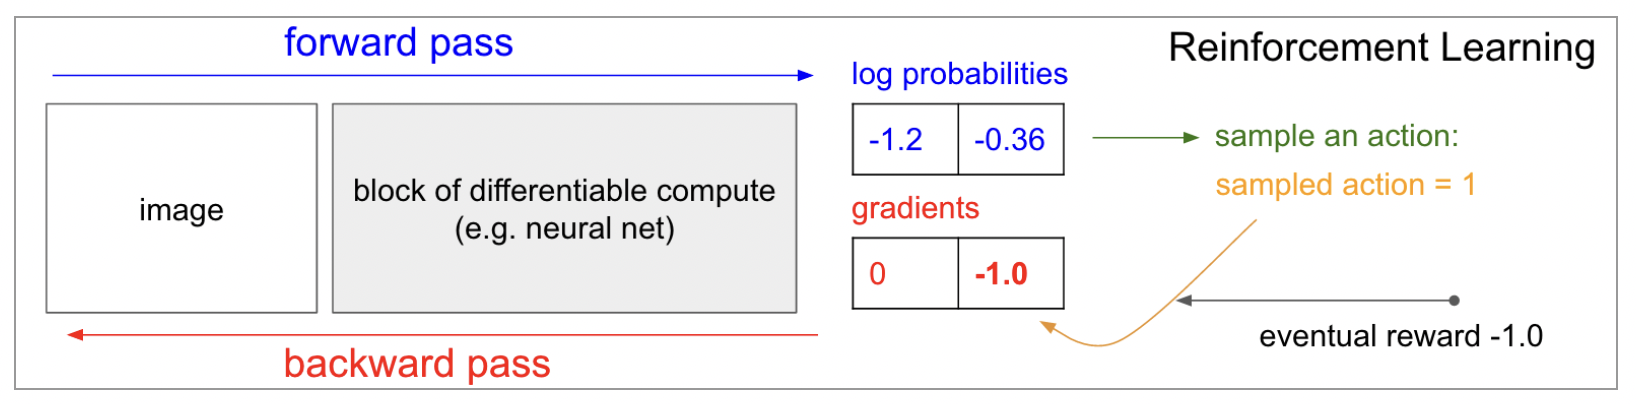
\includegraphics[width=1\textwidth]{policygrad.png} \\
	(note that this uses stochastic policy) 
\end{frame}

\begin{frame}
	\frametitle{Policy Gradient Methods}
	\center 
	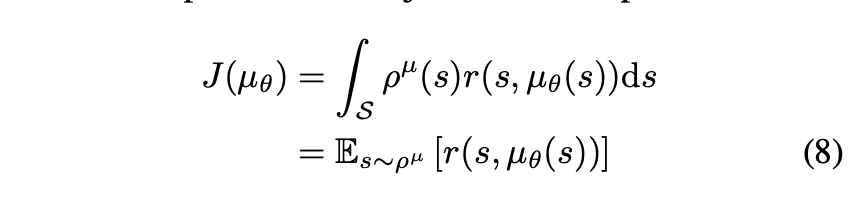
\includegraphics[width=1\textwidth]{performance.png} \\
	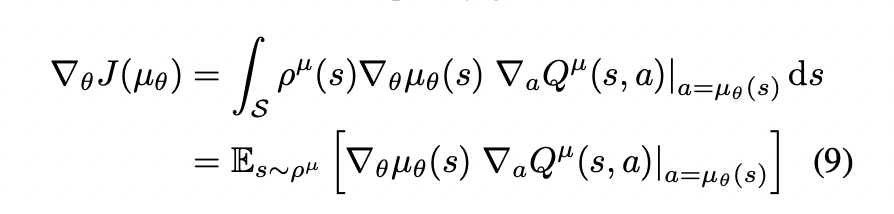
\includegraphics[width=1\textwidth]{gradient.png}
\end{frame}

\begin{frame}
	\frametitle{Actor-Critic}
	\center{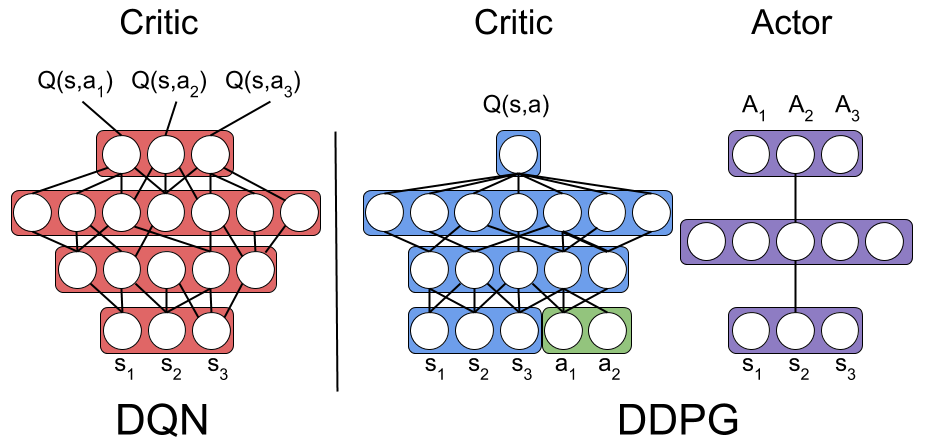
\includegraphics[width=0.6\textwidth]{dqn_ddpg_cropped.png}}
	\begin{itemize}
		\item 2 Networks: \\ 
			critic: (s, a) $\rightarrow$ V(s') \\
			actor: s $\rightarrow$ a \\
		\item Continuous Actions \\
		\item Action-Replay Buffer \\
		\item Target Network Updates
	\end{itemize}
\end{frame}

\begin{frame}
	\frametitle{Frameworks}
	\begin{itemize}
		\item OpenAI Gym \\
		\item PyTorch/Autograd \\
		\item OpenCV \\
		\item LibVirt
	\end{itemize}
\end{frame}

\begin{frame}
	\frametitle{Approach}
	\begin{itemize}
		\item[1] Set up environment \\	
		\item[2] Implement Deep \emph{Stochastic} Policy Gradient Algorithm \\
		\item[3] Add Replay Buffer, Target Network
		\item[4] Implement Actor-Critic For Deterministic Policy Gradient Algorithm
	\end{itemize}
\end{frame}
\begin{frame}
	\frametitle{References}
	\begin{itemize}
		\item DeepMind's 'Continuous Control with Deep Reinforcement Learning' (2016) \\
		\item DeepMind's 'Deterministic Policy Gradient Algorithms' (2014) \\
		\item DeepMind's 'Playing Atari with Deep Reinforcement Learning' (2015) \\
		\item Karpathy's 'Deep Reinforcement Learning: Pong from Pixels' (https://karpathy.github.io/2016/05/31/rl/)
	\end{itemize}
\end{frame}
\end{document}

